% Options for packages loaded elsewhere
% Options for packages loaded elsewhere
\PassOptionsToPackage{unicode}{hyperref}
\PassOptionsToPackage{hyphens}{url}
\PassOptionsToPackage{dvipsnames,svgnames,x11names}{xcolor}
%
\documentclass[
  11pt,
]{article}
\usepackage{xcolor}
\usepackage[top=0.4in,bottom=0.45in,left=0.65in,right=0.65in,includehead,headheight=52pt,headsep=7pt,includefoot,footskip=24pt]{geometry}
\usepackage{amsmath,amssymb}
\setcounter{secnumdepth}{-\maxdimen} % remove section numbering
\usepackage{iftex}
\ifPDFTeX
  \usepackage[T1]{fontenc}
  \usepackage[utf8]{inputenc}
  \usepackage{textcomp} % provide euro and other symbols
\else % if luatex or xetex
  \usepackage{unicode-math} % this also loads fontspec
  \defaultfontfeatures{Scale=MatchLowercase}
  \defaultfontfeatures[\rmfamily]{Ligatures=TeX,Scale=1}
\fi
\usepackage{lmodern}
\ifPDFTeX\else
  % xetex/luatex font selection
\fi
% Use upquote if available, for straight quotes in verbatim environments
\IfFileExists{upquote.sty}{\usepackage{upquote}}{}
\IfFileExists{microtype.sty}{% use microtype if available
  \usepackage[]{microtype}
  \UseMicrotypeSet[protrusion]{basicmath} % disable protrusion for tt fonts
}{}
\makeatletter
\@ifundefined{KOMAClassName}{% if non-KOMA class
  \IfFileExists{parskip.sty}{%
    \usepackage{parskip}
  }{% else
    \setlength{\parindent}{0pt}
    \setlength{\parskip}{6pt plus 2pt minus 1pt}}
}{% if KOMA class
  \KOMAoptions{parskip=half}}
\makeatother
% Make \paragraph and \subparagraph free-standing
\makeatletter
\ifx\paragraph\undefined\else
  \let\oldparagraph\paragraph
  \renewcommand{\paragraph}{
    \@ifstar
      \xxxParagraphStar
      \xxxParagraphNoStar
  }
  \newcommand{\xxxParagraphStar}[1]{\oldparagraph*{#1}\mbox{}}
  \newcommand{\xxxParagraphNoStar}[1]{\oldparagraph{#1}\mbox{}}
\fi
\ifx\subparagraph\undefined\else
  \let\oldsubparagraph\subparagraph
  \renewcommand{\subparagraph}{
    \@ifstar
      \xxxSubParagraphStar
      \xxxSubParagraphNoStar
  }
  \newcommand{\xxxSubParagraphStar}[1]{\oldsubparagraph*{#1}\mbox{}}
  \newcommand{\xxxSubParagraphNoStar}[1]{\oldsubparagraph{#1}\mbox{}}
\fi
\makeatother


\usepackage{longtable,booktabs,array}
\newcounter{none} % for unnumbered tables
\usepackage{calc} % for calculating minipage widths
% Correct order of tables after \paragraph or \subparagraph
\usepackage{etoolbox}
\makeatletter
\patchcmd\longtable{\par}{\if@noskipsec\mbox{}\fi\par}{}{}
\makeatother
% Allow footnotes in longtable head/foot
\IfFileExists{footnotehyper.sty}{\usepackage{footnotehyper}}{\usepackage{footnote}}
\makesavenoteenv{longtable}
\usepackage{graphicx}
\makeatletter
\newsavebox\pandoc@box
\newcommand*\pandocbounded[1]{% scales image to fit in text height/width
  \sbox\pandoc@box{#1}%
  \Gscale@div\@tempa{\textheight}{\dimexpr\ht\pandoc@box+\dp\pandoc@box\relax}%
  \Gscale@div\@tempb{\linewidth}{\wd\pandoc@box}%
  \ifdim\@tempb\p@<\@tempa\p@\let\@tempa\@tempb\fi% select the smaller of both
  \ifdim\@tempa\p@<\p@\scalebox{\@tempa}{\usebox\pandoc@box}%
  \else\usebox{\pandoc@box}%
  \fi%
}
% Set default figure placement to htbp
\def\fps@figure{htbp}
\makeatother





\setlength{\emergencystretch}{3em} % prevent overfull lines

\providecommand{\tightlist}{%
  \setlength{\itemsep}{0pt}\setlength{\parskip}{0pt}}



 


% =====================================================================
%  _style.tex  ·  Design system for EIL research highlights (v8 layout)
%  Edit here to restyle ALL research highlights. Included via the .qmd YAML.
%  Matches the canonical single-column v8 template; the masthead and footer
%  are set per-document via fancyhdr in each .qmd's include-in-header.
% =====================================================================

% ---- Colours (exact hex) --------------------------------------------
\definecolor{ink}{HTML}{1D2620}        % title, masthead rule
\definecolor{body}{HTML}{33352C}       % main body paragraphs
\definecolor{accentred}{HTML}{641111}  % RESEARCH HIGHLIGHT label, links, section heads, fig title
\definecolor{boxred}{HTML}{8C2826}     % Bottom Line box fill
\definecolor{boxtext}{HTML}{EEF1EA}    % Bottom Line body text (off-white)
\definecolor{muted}{HTML}{50534A}      % figure source line
\definecolor{cite}{HTML}{6E6D61}       % citation line
\definecolor{faint}{HTML}{9A978A}      % footer
\definecolor{warmrule}{HTML}{D8D2C2}   % thin warm-grey dividers
\definecolor{paper}{HTML}{FAF8F1}      % warm page background

% \pagecolor{paper}                    % uncomment for warm off-white background

% ---- Fonts (Source Sans 3 / Source Serif 4) -------------------------
\usepackage[T1]{fontenc}
\usepackage[default]{sourcesanspro}
\usepackage{sourceserifpro}
\renewcommand{\familydefault}{\sfdefault}

% ---- Page -----------------------------------------------------------
\pagestyle{empty}
\setlength{\parindent}{0pt}
\setlength{\parskip}{2pt}
% Default body size/colour. The .qmd overrides this to 10.5/13.5pt.
\AtBeginDocument{\color{body}\fontsize{9.4pt}{13.6pt}\selectfont}

% ---- Packages -------------------------------------------------------
\usepackage{microtype}
\usepackage{soul}
\setul{2pt}{.5pt}
\usepackage{tcolorbox}
\tcbuselibrary{skins}
\usepackage[colorlinks=true, urlcolor=accentred, linkcolor=accentred, pdfborder={0 0 0}]{hyperref}

% =====================================================================
%  MACROS
% =====================================================================

% --- Title + citation (citation has a thin warm divider beneath) ------
\newcommand{\brieftitle}[1]{%
  {\color{ink}\fontsize{18pt}{19.5pt}\selectfont\bfseries\textls[-12]{#1}\par}\vspace{3pt}}
\newcommand{\briefcitation}[1]{%
  {\color{cite}\fontsize{9.4pt}{12pt}\selectfont #1\par}\vspace{3pt}%
  \noindent\textcolor{warmrule}{\rule{\linewidth}{0.7pt}}}

% --- Section heads (uppercase, maroon) -------------------------------
\newcommand{\sectionhead}[1]{%
  \vspace{2pt}{\color{accentred}\bfseries\fontsize{9.75pt}{12pt}\selectfont
  \textls[20]{\MakeUppercase{#1}}\par}\vspace{1pt}}

% --- Sub-heads (small uppercase) -------------------------------------
% Legacy — the retired Takeaways block used these. Kept in the brand
% maroon so older highlights that call \subhead still compile.
\newcommand{\subhead}[1]{%
  {\color{accentred}\bfseries\fontsize{8.25pt}{10pt}\selectfont
  \textls[50]{\MakeUppercase{#1}}\par}\vspace{2pt}}

% --- Figure title + source line --------------------------------------
\newcommand{\figtitle}[2]{%
  {\bfseries\color{accentred}\fontsize{7.1pt}{9pt}\selectfont\textls[40]{\MakeUppercase{#1}}}\par%
  {\color{muted}\fontsize{7.1pt}{9pt}\selectfont #2}\par\vspace{4pt}}

% =====================================================================
%  COLOURED BOXES
% =====================================================================

% --- Bottom Line box (border-radius 6px -> arc=4pt) ------------------
\newtcolorbox{bottomline}{%
  enhanced, arc=4pt, outer arc=4pt, boxrule=0pt,
  colback=boxred, coltext=boxtext,
  left=7pt, right=7pt, top=7pt, bottom=7pt,
  before upper={\fontsize{9.4pt}{13.6pt}\selectfont}}

% --- Info box (contact + full citation; centered, thin faint border) --
% Superseded by the moreinfo environment below; kept so older highlights
% still compile. Faint text at footer size. Wrap any link as
% \href{url}{\color{faint}\underline{text}} so it inherits the faint
% colour instead of the global accent link colour.
\newtcolorbox{infobox}{%
  enhanced, width=0.9\linewidth, center, arc=4pt, outer arc=4pt,
  boxrule=0.5pt, colframe=faint, colback=white, coltext=faint,
  left=9pt, right=9pt, top=7pt, bottom=7pt,
  before upper={\fontsize{7.4pt}{9.5pt}\selectfont}}

% =====================================================================
%  CLOSING BLOCK
% =====================================================================

% --- For more information (full width; rule above, no box) ------------
% Four paragraphs: contact line, full citation, author affiliations
% (one bold-lead sentence each), then the EIL boilerplate. Wrap any link as
% \href{url}{\color{cite}\underline{text}} so it inherits the block's
% grey instead of the global accent link colour.
\newenvironment{moreinfo}{%
  \par\vspace{12pt}%
  \noindent\textcolor{warmrule}{\rule{\linewidth}{0.7pt}}\par
  \vspace{7pt}%
  {\color{ink}\bfseries\fontsize{8.25pt}{10pt}\selectfont
   \textls[50]{\MakeUppercase{For more information}}\par}\vspace{4pt}%
  \color{cite}\fontsize{8.4pt}{11.5pt}\selectfont
  \setlength{\parskip}{5pt}%
}{\par}
% --- Background wrap figure ---
\usepackage{wrapfig}
% --- Running masthead + footer (logo, label, rule, page number) ---
\usepackage{fancyhdr}
\renewcommand{\headrulewidth}{0pt}
\renewcommand{\footrulewidth}{0pt}
\fancypagestyle{brief}{%
  \fancyhf{}%
  \fancyhead[L]{%
    \begin{minipage}[c]{0.62\textwidth}\raggedright\color{ink}\includegraphics[height=0.45in]{../../../formats/logos/eil-logo-maroon.png}\end{minipage}\hfill%
    \begin{minipage}[c]{0.36\textwidth}\raggedleft\fontsize{8.25pt}{10pt}\selectfont\bfseries\color{accentred}\textls[200]{\MakeUppercase{Research Highlight}}\end{minipage}%
    \par\vspace{2pt}%
    \noindent\textcolor{ink}{\rule{\textwidth}{2.2pt}}%
  }%
  \fancyfoot[C]{%
    \color{warmrule}\rule{\textwidth}{0.7pt}\par\vspace{3pt}%
    \hbox to\textwidth{%
      \color{faint}\fontsize{7.4pt}{9pt}\selectfont
      For full paper:\hspace{0.4em}\href{[NBER working paper link — add once available]}{\color{faint}\underline{\textls[40]{[nber.org/papers/... — add once available]}}}%
      \hfill
      Page \thepage%
    }%
  }%
}
\pagestyle{brief}
\makeatletter
\@ifpackageloaded{caption}{}{\usepackage{caption}}
\AtBeginDocument{%
\ifdefined\contentsname
  \renewcommand*\contentsname{Table of contents}
\else
  \newcommand\contentsname{Table of contents}
\fi
\ifdefined\listfigurename
  \renewcommand*\listfigurename{List of Figures}
\else
  \newcommand\listfigurename{List of Figures}
\fi
\ifdefined\listtablename
  \renewcommand*\listtablename{List of Tables}
\else
  \newcommand\listtablename{List of Tables}
\fi
\ifdefined\figurename
  \renewcommand*\figurename{Figure}
\else
  \newcommand\figurename{Figure}
\fi
\ifdefined\tablename
  \renewcommand*\tablename{Table}
\else
  \newcommand\tablename{Table}
\fi
}
\@ifpackageloaded{float}{}{\usepackage{float}}
\floatstyle{ruled}
\@ifundefined{c@chapter}{\newfloat{codelisting}{h}{lop}}{\newfloat{codelisting}{h}{lop}[chapter]}
\floatname{codelisting}{Listing}
\newcommand*\listoflistings{\listof{codelisting}{List of Listings}}
\makeatother
\makeatletter
\makeatother
\makeatletter
\@ifpackageloaded{caption}{}{\usepackage{caption}}
\@ifpackageloaded{subcaption}{}{\usepackage{subcaption}}
\makeatother
\usepackage{bookmark}
\IfFileExists{xurl.sty}{\usepackage{xurl}}{} % add URL line breaks if available
\urlstyle{same}
\hypersetup{
  colorlinks=true,
  linkcolor={blue},
  filecolor={Maroon},
  citecolor={Blue},
  urlcolor={Blue},
  pdfcreator={LaTeX via pandoc}}


\author{}
\date{}
\begin{document}


% ---------------------------------------------------------------------
% TITLE + CITATION  (masthead repeats in the page header)
% ---------------------------------------------------------------------
\brieftitle{Losing a home in a wildfire costs more than just the rebuild}
\briefcitation{Lessons from ``The Distribution and Consequences of Natural Disasters: Evidence from U.S. Wildfire Victims'' by Patrick Baylis, Judson Boomhower, Jonathan Colmer, and John Voorheis, NBER Working Paper, 2026.}

\vspace{-2pt}

% override body font size for this document
\fontsize{10.5pt}{13.5pt}\selectfont

% ---------------------------------------------------------------------
% BOTTOM LINE  (~40–50 words)
% ---------------------------------------------------------------------
\begin{bottomline}
{\fontsize{11pt}{15pt}\selectfont
New research studying nearly all wildfires in the past 25 years shows that \textbf{when a wildfire destroys a home, occupants don't just lose the structure — they lose income too, for years afterward.} 
}
\end{bottomline}

\vspace{6pt}

% ---------------------------------------------------------------------
% BACKGROUND  (~120 words, 2 paragraphs)
% ---------------------------------------------------------------------
\sectionhead{Background}
% TODO — Background figure not yet built: recreate Fig. 1 (Glass Fire map of
% destroyed/surviving/adjacent homes) or Fig. 2 (pre-fire income distribution,
% destroyed vs. surviving). Confirm estimates with Grant before scripting it.
\begin{wrapfigure}{r}{3.85in}
  \vspace{-\intextsep}
  \centering
  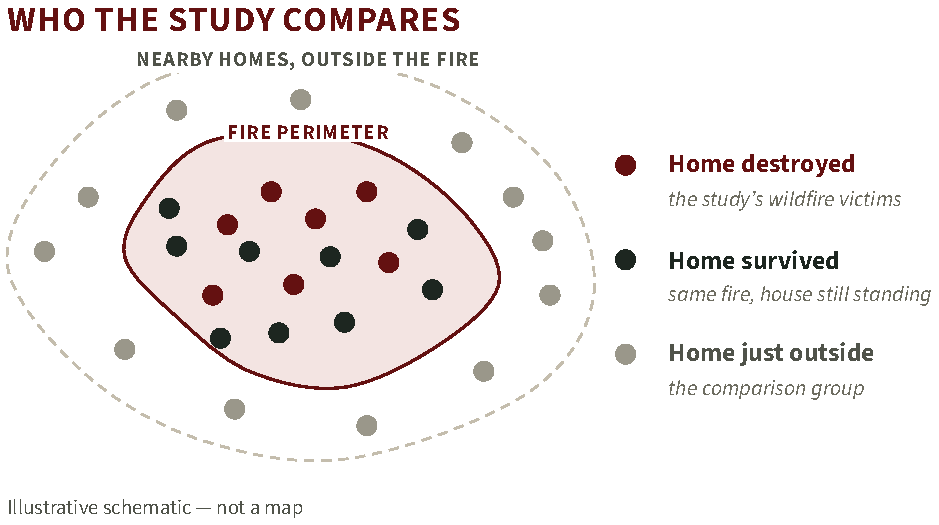
\includegraphics[width=3.85in]{../data-viz/figures/fig-comparison-groups.pdf}
\end{wrapfigure}
\hyphenpenalty=10000 \exhyphenpenalty=10000
\noindent Global economic losses from natural catastrophes totaled \$320 billion in 2024. Though this number is striking, it masks that \textbf{the financial consequences of disasters are unevenly distributed across households.} To respond well to disasters, it's important to know who bears the losses, whether the damage to household finances goes beyond the cost of rebuilding, and what happens to a neighborhood as it recovers. This is especially true for areas prone to wildfires, which are increasing in frequency and severity.

\noindent \textbf{In a new working paper, Baylis et al. (2026) find that those whose homes were destroyed in a wildfire don't just lose the value of their house, they also lose a significant portion of their income for years afterward.} The researchers studied nearly all catastrophic wildfires in the United States from 2003 to 2022 and analyzed property damage alongside occupant demographics and income data.
\hyphenpenalty=50 \exhyphenpenalty=50

\vspace{6pt}

% ---------------------------------------------------------------------
% THE CHALLENGE  (~180–300 words) — the research-design story
% ---------------------------------------------------------------------
\sectionhead{The challenge}
\noindent \textbf{Measuring what a wildfire costs the people in its path is harder than it looks.} Comparing a household's income before and after the fire risks crediting the fire with changes already underway in the local economy.

\noindent Comparing wildfire victims to people elsewhere raises a different concern: fires strike particular places, and the households in their path were already wealthier and older than the country as a whole. Narrowing to a single fire — setting households whose homes burned against neighbors whose homes came through standing — puts both groups in the same place at the same moment. Homes did not survive at equal rates, however: those that burned belonged to lower-income households than those left standing, so the two groups differed before the fire started.

\noindent \textbf{Baylis et al. instead tracked the two groups separately, comparing each against people living just outside the fire's perimeter.} These neighbors shared the same local job market, so whatever moved incomes across the area moved them for everyone. Before each fire, all three groups' incomes rose and fell together, supporting their use as a stand-in for what victims would have earned had the fire never reached them.

\vspace{6pt}

% ---------------------------------------------------------------------
% FINDINGS  (~150 words + figure)
% ---------------------------------------------------------------------
\sectionhead{Income fell only for those who lost a home}
\noindent Households whose homes were destroyed earned less than their neighbors just outside the perimeter for three years running — about 11\% less at the low point in the second year, before catching back up by the fourth (see figure). Added up, the shortfall comes to roughly 30\% of a single year's pre-fire income, or about \$38,000, on top of what the rebuild itself cost. Households whose homes survived the same fires barely departed from those neighbors at all. \textbf{The loss tracks whose house burned, not who lived through the fire.}

\vspace{6pt}

\begin{center}
\begin{minipage}{0.75\linewidth}
\figtitle{The wildfire's effect on income, year by year}{Source: Baylis, Boomhower, Colmer \& Voorheis (2026), Fig.\ 4a.}
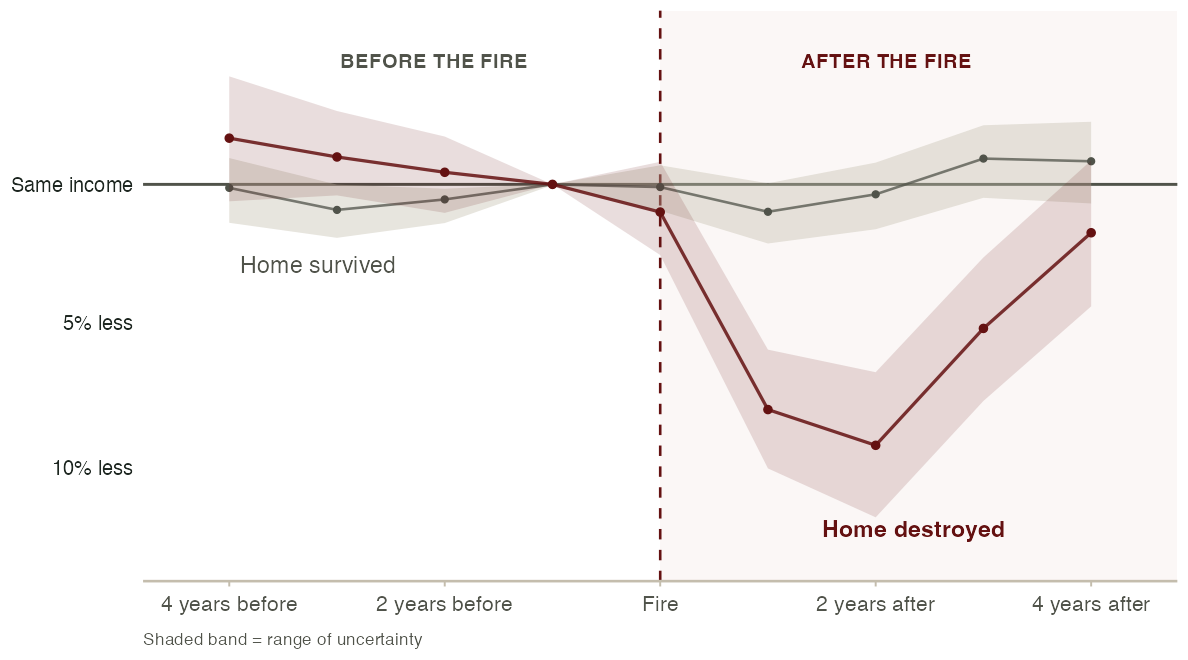
\includegraphics[width=\linewidth]{../data-viz/figures/fig1-income-by-damage.png}
\par\vspace{3pt}
{\color{faint}\fontsize{7.1pt}{9.5pt}\selectfont \textit{Note:} This figure shows the estimated effect of a wildfire on the incomes of people who lived inside its perimeter. One line follows occupants whose homes were destroyed; the other follows occupants of homes in the same fires that survived. Both are measured against similar people who lived just outside the perimeter, and both are set to zero in the year before the fire. A point below the line means that group had fallen behind those outside neighbors. The estimates account for occupants' characteristics and for anything that affected everyone caught in the same fire in the same year. If living through a fire, rather than losing a home to the fire, is what costs people income, both of the lines would fall after the fire. \par}
\end{minipage}
\end{center}

\vspace{6pt}

% ---------------------------------------------------------------------
% IMPLICATIONS FOR POLICY  (~120 words, ~2 paragraphs)
% ---------------------------------------------------------------------
\sectionhead{Implications for policy}
\noindent Wildfire loss in the U.S. is often pictured as a wealthy Californian's problem. These households were better off than the country as a whole on average, though within a single fire it was the lower-income homes that burned --- and a quarter of the people who lost one earned under \$42,000.

\noindent Four years after a fire, half of destroyed addresses are still unoccupied, and the homes that do come back tend to house higher-income, younger residents than those who lived there before. \textbf{Recovery aid measured by how fast a neighborhood rebuilds can miss whether the people who lost their homes are the ones who return.}

\noindent This is one set of large U.S. wildfires between 2003 and 2022, and the paper does not settle why income falls. What it does establish is the size of the loss: enough that \textbf{helping households protect a home before a fire may be worth more than it appears when only the structure is counted.}

\vspace{6pt}

% ---------------------------------------------------------------------
% FOR MORE INFO
% ---------------------------------------------------------------------
% GUIDANCE: corresponding author/contact not stated in the paper — confirm
% with the author team before publishing. Titles/ranks below are left
% blank intentionally (not stated in the paper) — fill in once confirmed.
\begin{moreinfo}
Contact [Corresponding author] ([email]) with questions about this research.\par

Baylis, Patrick, Judson Boomhower, Jonathan Colmer, and John Voorheis. 2026. ``The Distribution and Consequences of Natural Disasters: Evidence from U.S. Wildfire Victims.'' NBER Working Paper. \href{[NBER working paper link — add once available]}{\color{cite}\underline{[nber.org/papers/... — add once available]}}.\par

\textbf{Patrick Baylis} is [title] at the Vancouver School of Economics, University of British Columbia.\par
\textbf{Judson Boomhower} is [title] in the Department of Economics at the University of California San Diego, and [status] at NBER.\par
\textbf{Jonathan Colmer} is [title] in the Department of Economics at the University of Virginia.\par
\textbf{John Voorheis} is [title] at the Center for Economic Studies, U.S. Census Bureau.\par

The \href{https://www.environmental-inequality-lab.org/}{\color{cite}\underline{Environmental Inequality Lab}} is a nonpartisan research group that applies a rigorous, data-driven approach to understand how our environment shapes economic opportunity and well-being.\par
\end{moreinfo}




\end{document}
